\documentclass[11pt,a4paper]{article}

\usepackage[T1]{fontenc}
\usepackage[utf8]{inputenc}
\usepackage{lmodern}
\usepackage{microtype}
\usepackage[skip=5pt plus 1pt]{parskip}
\usepackage[margin=25mm]{geometry}
\usepackage[table]{xcolor}
\usepackage{amsmath,amssymb}
\usepackage{graphicx}
\usepackage{booktabs}
\usepackage{enumitem}
\usepackage{caption}
\usepackage{titlesec}
\usepackage{tcolorbox}
\usepackage[normalem]{ulem}
% prebuilt figures/*.pdf when present (see Makefile), else compiled inline
\usepackage[mode=image|tex]{standalone}
\usepackage{tikz}
\usetikzlibrary{arrows.meta,calc,positioning,decorations.pathmorphing}
\usepackage[hidelinks]{hyperref}

%% ---------------------------------------------------------------- styling
\definecolor{rcrblue}{RGB}{0,102,170}
\definecolor{rcrorange}{RGB}{214,84,58}

\titleformat{\section}{\Large\bfseries\color{rcrblue}}{\thesection}{0.7em}{}
\titleformat{\subsection}{\large\bfseries}{\thesubsection}{0.6em}{}
\captionsetup{font=small,labelfont={bf,color=rcrblue}}
\setlist[itemize]{leftmargin=1.4em,itemsep=2pt,topsep=3pt}
\setlist[enumerate]{leftmargin=1.6em,itemsep=2pt,topsep=3pt}

%% ---------------------------------------------------------------- review
%% Changes not yet reviewed are highlighted in yellow.
%% \reviewtrue shows the highlights; switch to \reviewfalse once reviewed.
\newif\ifreview
\reviewtrue
\definecolor{chg}{RGB}{255,240,110}
\tcbuselibrary{breakable}
\newtcolorbox{changed}{breakable,colback=chg,colframe=chg,boxrule=0pt,
  arc=0pt,outer arc=0pt,left=0pt,right=0pt,top=1pt,bottom=1pt,
  grow to left by=2pt,grow to right by=2pt,before skip=2pt,after skip=2pt,
  before upper={\parskip=5pt plus 1pt}}
\ifreview\else\renewenvironment{changed}{}{}\fi
%% deleted text: shown struck through while under review, gone otherwise
\newcommand{\del}[1]{\ifreview\begin{changed}\textcolor{black!55}{\sout{#1}}\end{changed}\fi}
%% changed inline words
\newcommand{\chg}[1]{\ifreview\colorbox{chg}{#1}\else#1\fi}
%% changed table row
\newcommand{\chgrow}{\ifreview\rowcolor{chg}\fi}
%% changed figure: yellow frame
\newcommand{\chgfig}[1]{\ifreview{\setlength{\fboxrule}{2.5pt}%
  \fcolorbox{chg}{white}{#1}}\else#1\fi}

%% time factors: colour scale green (x1) -> orange -> red (x1.5)
\definecolor{tfA}{RGB}{34,153,84}   % x1
\definecolor{tfB}{RGB}{116,148,50}  % x1.1
\definecolor{tfC}{RGB}{235,135,0}   % x1.25
\definecolor{tfD}{RGB}{210,40,40}   % x1.5
\newcommand{\tf}[2]{\textcolor{#1}{\bfseries$\boldsymbol{\times}$#2}}

%% open point, inline
\newcommand{\tbd}[1]{\textcolor{rcrorange}{\textbf{[TBD%
  \if\relax\detokenize{#1}\relax\else: #1\fi]}}}

%% open point, block
\newtcolorbox{openpoint}[1][Open point]{%
  colback=rcrorange!5,colframe=rcrorange!70,coltitle=white,
  fonttitle=\bfseries\small,title={#1},boxrule=0.6pt,arc=2pt,
  left=5pt,right=5pt,top=4pt,bottom=4pt}


%% rules revision -- bump on every published change
%% (the release workflow overrides it with the release tag)
\providecommand{\rulesrev}{rev0}
\hypersetup{pdftitle={Rock Climbing Robots \textemdash\ Rules \rulesrev}}

\usepackage{fancyhdr}
\pagestyle{fancy}
\fancyhf{}
\renewcommand{\headrulewidth}{0pt}
\fancyfoot[L]{\small\textcolor{black!55}{Rock Climbing Robots --- Rules \rulesrev}}
\fancyfoot[R]{\small\thepage}
\fancypagestyle{plain}{\fancyhf{}\fancyfoot[L]{\small\textcolor{black!55}{Rock Climbing Robots --- Rules \rulesrev}}\fancyfoot[R]{\small\thepage}}

\title{\vspace{-12mm}\textbf{Rock Climbing Robots}\\[2mm]
       \large Hackathon Rulebook --- \emph{Draft}}
\author{}
\date{Rules revision \textbf{\rulesrev} --- \today}

\begin{document}
\maketitle
\vspace{-8mm}

\begin{center}
\begin{tcolorbox}[colback=rcrorange!5,colframe=rcrorange!60,boxrule=0.6pt,arc=2pt,
                  width=0.92\textwidth,left=6pt,right=6pt,top=4pt,bottom=4pt]
\small\textbf{Draft document.} Every item marked \tbd{\dots} or listed in an
\emph{Open point} box still has to be decided before the rules are frozen.
\end{tcolorbox}
\end{center}

\tableofcontents
\bigskip

%% ================================================================
\section{Overview}

\textbf{Rock Climbing Robots} is a hackathon in which teams design, build and
program small legged robots that climb an instrumented artificial climbing
wall. Each robot is secured by a safety rope running over a pulley at the top
of the wall, exactly as a human climber would be.

\medskip
\noindent\textbf{Website:} \url{https://rock-climbing-robots.github.io/}
\medskip

The event combines mechanical design (limbs, grippers, anchor point), control
(balance and contact planning on a sparse set of holds) and perception (two
external cameras observe the wall).

\begin{itemize}
  \item \textbf{Teams:} 2 to 6 members per team.
  \item \textbf{Deliverable:} a robot able to climb from the start zone to the
        top of the wall using the mounted holds.
  \item \textbf{Scoring:} two independent evaluations, in simulation and on
        the real robot (Section~\ref{sec:scoring}).
\end{itemize}

%% ================================================================
\section{Robots}

\subsection{Morphology}

The robot climbs using its \emph{limbs}; its shape is otherwise not
constrained. Other parts of the robot, such as its trunk, may also touch the
wall and the holds.

A \emph{humanoid} robot has \textbf{four limbs}: a central trunk carrying two
upper limbs and two lower limbs. Whether a robot is humanoid is left to the
discretion of the organisers. Non-humanoid robots are allowed, with a time
factor (Section~\ref{sec:scoring}).

Attachment to the wall must be made through the holds.

\subsection{Size}

The maximum height of the robot is \textbf{400\,mm}, measured with the
robot standing in its nominal upright posture, arms along the body.

Limbs may extend beyond that envelope while climbing; the 400\,mm limit
applies to the reference posture only.

There is \textbf{no limit} on the width or the depth of the robot.

The mass of the robot must not exceed \textbf{2\,kg}.

\subsection{Power}

A robot may be powered either:
\begin{enumerate}[label=(\alph*)]
  \item by \textbf{on-board batteries}, or
  \item by an \textbf{external power supply}, whose cable is routed along the
        safety rope down to the robot (see Section~\ref{sec:setup}).
\end{enumerate}

A tethered cable must be attached to the safety rope and must never be
load-bearing: it shall not be able to hold the robot if the anchor point fails, and
it shall not be used to help the robot climb.

\subsection{Control and autonomy}

Computation may be on-board or off-board.
Communication with external computers is free: the Ethernet tether or any
wireless link (Wi-Fi, Bluetooth, etc.), on any band, may be used.

The robot must be \textbf{autonomous}: \textbf{teleoperation is not allowed}.

\subsection{Provided robots}

Robots will be provided by the organisers to teams that do not bring their
own platform.

The provided platform is derived from \textbf{Microban}, an open-source,
fully 3D-printable humanoid robot of about 30\,cm developed by the Rhoban team
(LaBRI, University of Bordeaux), with \textbf{limbs adapted for climbing}.

\begin{center}
\small
\begin{tabular}{@{}ll@{}}
\toprule
\textbf{Item} & \textbf{Value}\\
\midrule
Actuators          & $19\times$ Dynamixel \texttt{XL330-M288-T}\\
Degrees of freedom & 6 per leg, 3 per arm\\
Height             & $\approx 300$\,mm (base Microban)\\
Repository         & \url{https://github.com/Rhoban/microban}\\
\bottomrule
\end{tabular}
\end{center}

\begin{figure}[h!]
  \centering
  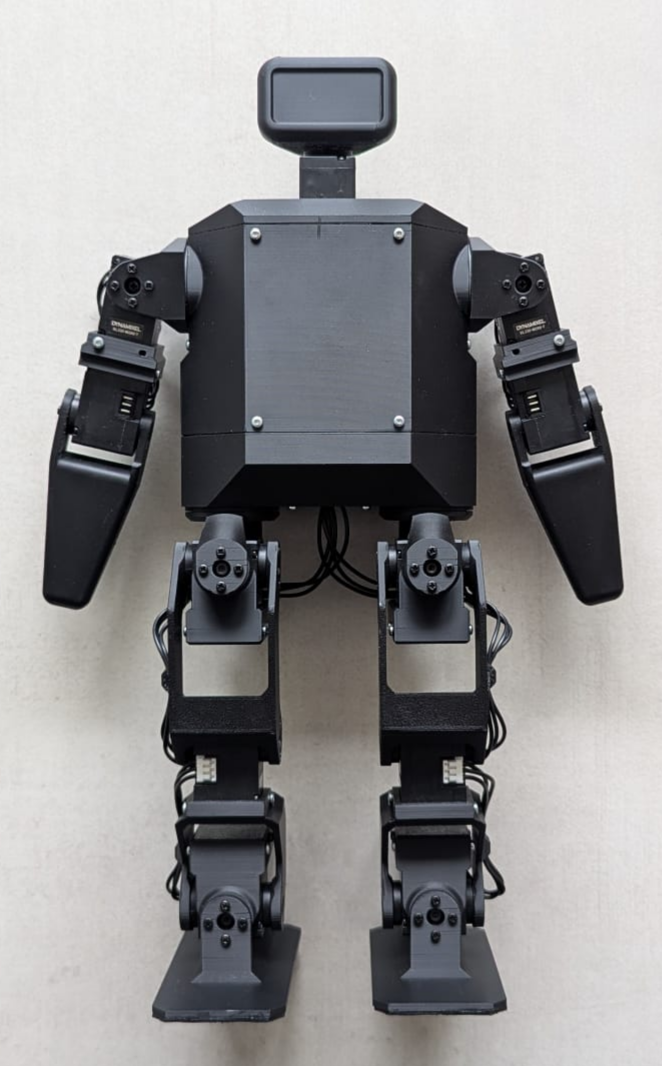
\includegraphics[height=62mm]{figures/img/microban_front}\hspace{10mm}
  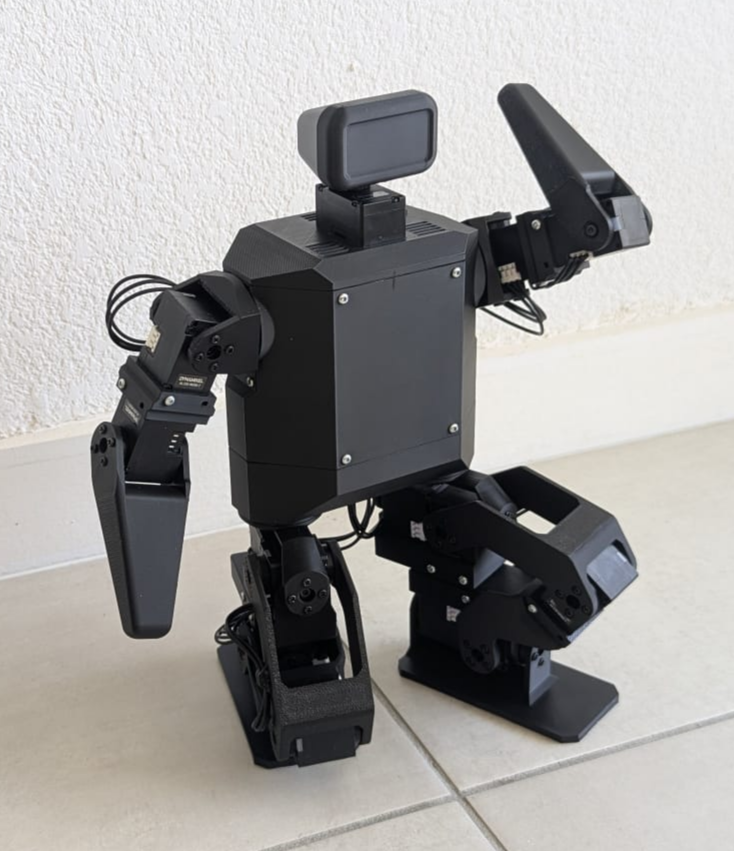
\includegraphics[height=62mm]{figures/img/microban_side}
  \caption{\textbf{Microban}, the base platform for the provided robots, shown
           here in its standard configuration --- the climbing version uses
           adapted limbs. Photographs from the Microban repository
           (Rhoban team, LaBRI, University of Bordeaux).}
  \label{fig:microban}
\end{figure}

\begin{openpoint}[To be specified --- provided robot]
Quantity available, on-board computer and SDK, allocation of the 19th servo
(6\,DOF $\times$ 2 legs $+$ 3\,DOF $\times$ 2 arms $= 18$; the remaining one is
presumably the trunk or the head), and which mechanical modifications are
allowed on the provided robots.
\end{openpoint}

%% ================================================================
\section{Climbing wall}
\label{sec:wall}

\textbf{Four walls} are provided by the organisers. The boards are identical:
the difficulty comes from the configuration of the holds, which are
reconfigured during the event. There are \textbf{three difficulty levels}:
\begin{itemize}
  \item \textbf{Level 1} --- a ``ladder'': regularly spaced holds;
  \item \textbf{Level 2} --- a ladder with missing holds;
  \item \textbf{Level 3} --- the robot needs to move to the right or to the left.
\end{itemize}

Each climbing wall is a flat rectangular board, mounted vertically, of
\textbf{1400\,mm} height and \textbf{800\,mm} width.

The board is made of a \textbf{sturdy material} (for example MDF or CTM), with
a thickness of \textbf{10\,mm}, mounted on a rigid frame.

The board is drilled with a regular square grid of \textbf{M3} holes with
a pitch of \textbf{15\,mm}. The border margin is 10\,mm on all four sides.
Holes are plain through-holes: holds are bolted from the front and
tightened by nuts on the rear side of the board.

\begin{figure}[h!]
  \centering
  \includestandalone[width=0.92\textwidth]{figures/wall}
  \caption{Climbing wall --- front and side views. All dimensions in
           millimetres. Hole positions are shown enlarged for readability.}
  \label{fig:wall}
\end{figure}

\begin{openpoint}[To be confirmed --- wall]
\begin{itemize}
  \item Surface finish (raw, painted, varnished) --- this changes friction
        significantly.
\end{itemize}
\end{openpoint}

%% ================================================================
\section{Holds}
\label{sec:holds}

Holds compatible with the climbing variant of the Microban platform are
provided by the organisers.

Teams may come with \textbf{their own holds}, or adapt the provided ones, as
long as they remain compatible with the wall format (Figure~\ref{fig:hold}):
\begin{itemize}
  \item a hold is fixed with \textbf{two M3 bolts}, on \textbf{two holes side
        by side horizontally} on the grid, i.e.\ \textbf{15\,mm apart}; the bolts go through the hold
        and the board, and are tightened by \textbf{nuts on the opposite side
        of the wall};
  \item a hold must fit inside a \textbf{cylinder of diameter 60\,mm (radius 30\,mm) and length
        100\,mm}, whose axis is normal to the wall and centred between the two
        bolts.
\end{itemize}

\begin{figure}[h!]
  \centering
  \includestandalone[width=0.97\textwidth]{figures/hold}
  \caption{Hold specification: two M3 bolts on horizontally adjacent grid holes, passing
           through the hold and the board and tightened by nuts on the rear of
           the wall, and the cylindrical envelope ($\varnothing=60$\,mm, $L=100$\,mm) the
           hold must fit in. All dimensions in millimetres.}
  \label{fig:hold}
\end{figure}

%% ================================================================
\section{Setup}
\label{sec:setup}

The complete setup around one wall is shown in Figure~\ref{fig:setup}.

\begin{figure}[h!]
  \centering
  \includestandalone[width=\textwidth]{figures/setup}
  \caption{Isometric view of the setup: instrumented wall, crossbeam and
           pulley, safety rope with the optional Ethernet\,/\,power tether, and
           the two external USB cameras observing the wall.}
  \label{fig:setup}
\end{figure}

\subsection{Cameras}

Two external cameras are available per wall, one on each side, connected
over \textbf{USB}. They are provided and positioned by the organisers.

It is up to the teams to \textbf{plug the USB cables} into their own computer
and to \textbf{retrieve the images}. Teams must only use the \textbf{RGB
components} of the camera streams.

Both cameras observe the full wall surface. Their images are available to
the teams for perception and for run recording.

\subsection{ArUco markers}
\label{sec:aruco}

\textbf{ArUco markers are provided by the organisers}, ready to be attached
to the \textbf{four corners} of the wall.

Each wall marker (Figure~\ref{fig:aruco}) is:
\begin{itemize}
  \item a square \textbf{black code of $100\times100$\,mm},
  \item surrounded by a \textbf{white border of 18\,mm}, i.e.\
        $136\times136$\,mm in total,
  \item placed so that the \textbf{outer corner of the white border coincides
        with the corner of the wall}.
\end{itemize}

The marker IDs are:

\begin{center}
\small
\begin{tabular}{@{}cl@{}}
\toprule
\textbf{ID} & \textbf{Position}\\
\midrule
1 & top-left corner of the wall\\
2 & top-right corner of the wall\\
3 & bottom-left corner of the wall\\
4 & bottom-right corner of the wall\\
5 & robot\\
\bottomrule
\end{tabular}
\end{center}

The wall markers give the cameras their extrinsic parameters with respect
to the wall frame, and therefore a common reference frame for all teams.

A team may attach \textbf{marker ID~5 on its robot}, \textbf{wherever it wants}
on the robot and with the \textbf{size of its choice}, to be tracked by the
external cameras.

All markers belong to the ArUco dictionary \textbf{\texttt{DICT\_4X4\_50}}.
\begin{figure}[h!]
  \centering
  \includestandalone[width=0.8\textwidth]{figures/aruco}
  \caption{ArUco marker ID~1 at the top-left corner of the wall: $100\times100$\,mm
           black code, $18$\,mm white border, outer corner of the border on the
           wall corner. The other corners are symmetric. Dimensions in
           millimetres.}
  \label{fig:aruco}
\end{figure}

\subsection{Tether: Ethernet and power}

Ethernet and power cables may be attached along the safety rope. They must
follow the rope and must not be routed to a separate anchor point.

Cable strain relief must be provided on the robot side so that a fall
loads the anchor point, never the connectors.

\subsection{Anchor point}

Each team must provide on its robot an \textbf{anchor point for the safety
rope}.

%% ================================================================
\section{Perception}
\label{sec:perception}

Each run is performed in one of two perception modes. The mode only depends on
whether ArUco markers are used; it determines the time factor applied in the
ranking (Section~\ref{sec:scoring}).

\subsection{With ArUco markers}

The ArUco markers are attached to the four corners of the wall
(Section~\ref{sec:aruco}). They give the \textbf{extrinsic parameters of the
external cameras}, i.e.\ the pose of each camera with respect to the wall.

The robot may then be:
\begin{itemize}
  \item \textbf{tracked with its own ArUco marker}
        (ID~5), attached by the team
        (Section~\ref{sec:aruco}): the robot pose in the wall frame is given
        directly by marker detection;
  \item or \textbf{detected without a marker on the robot}, e.g.\ by a learned
        model, the wall markers still providing the camera extrinsics.
\end{itemize}

\subsection{Markerless}

\textbf{No ArUco marker} is present, neither on the wall nor on the robot. The
wall, the holds and the robot are perceived \emph{naturally} from the camera
images.

\textbf{The camera extrinsics are not given.} At the start of each attempt,
the organisers \textbf{slightly move the external cameras}; estimating the
pose of the cameras with respect to the wall is the job of the team's code.

\subsection{On-board vision}

The robot may also use its own on-board camera(s), alone or together with the
external cameras. The same two modes apply: the run is \emph{with ArUco
markers} if markers are used, \emph{markerless} otherwise.

%% ================================================================
\section{Simulation}
\label{sec:simulation}

In addition to the real robot, teams are evaluated in simulation, using the
\textbf{MuJoCo} physics simulator.

\textbf{A simulator will be provided by the organisers} at a later date. It is
based on \textbf{MuJoCo (CPU)} and includes the models of the \textbf{robot},
the \textbf{walls} and the \textbf{holds}.

\begin{itemize}
  \item The simulated competition uses walls of the \textbf{same
        three difficulty levels} as the real one.
  \item \textbf{Perception is simulated by MuJoCo}: the robot relies on the
        camera images rendered by the simulator. The two perception modes of
        Section~\ref{sec:perception} (with ArUco markers, markerless) apply in
        the same way, with the same time factors.
  \item Runs in simulation are ranked with the same rules as on the real
        robot (Section~\ref{sec:scoring}).
\end{itemize}

\begin{openpoint}[To be specified --- simulation]

Release date of the simulator; simulated cameras (placement, resolution,
rendering of the ArUco markers, displacement of the cameras for markerless
runs); how and on which hardware the simulated runs are executed for the
official evaluation.
\end{openpoint}

%% ================================================================
\section{Evaluation and scoring}
\label{sec:scoring}

There are \textbf{two completely independent evaluations}, each with its own
ranking: \textbf{in simulation} and \textbf{on the real robot}. Both use walls
of three difficulty levels. The goal is to \textbf{climb the wall in the
shortest time}.

\textbf{Start of a run.} The robot is either placed \emph{on the ground},
anywhere around the wall, and gets onto the wall by itself; or placed \emph{at
the bottom of the wall}.

\textbf{Height climbed.} The height climbed is given by the \textbf{highest hold
touched} by the robot. \textbf{Reaching the top} of the wall means touching one
of the \textbf{highest holds}.

\textbf{Ranking.} Runs are compared by:
\begin{enumerate}[leftmargin=1.8em]
  \item \textbf{height climbed} --- higher always beats lower, whatever the
        time;
  \item \textbf{time}, multiplied by the factors below.
\end{enumerate}

\begin{center}
\small
\begin{tabular}{@{}lc@{}}
\toprule
\textbf{Condition} & \textbf{Time factor}\\
\midrule
Wall difficulty level 3 & \tf{tfA}{1}\\
Wall difficulty level 2 & \tf{tfC}{1.25}\\
Wall difficulty level 1 & \tf{tfD}{1.5}\\
\midrule
Start on the ground, robot gets onto the wall by itself & \tf{tfA}{1}\\
Start at the bottom of the wall                         & \tf{tfB}{1.1}\\
\midrule
Markerless perception                                   & \tf{tfA}{1}\\
Perception using ArUco markers                          & \tf{tfC}{1.25}\\
\midrule
Humanoid robot                                  & \tf{tfA}{1}\\
Non-humanoid robot                              & \tf{tfB}{1.1}\\
\bottomrule
\end{tabular}
\end{center}

Factors multiply: for instance, a run on a level-2 wall, starting at the bottom
of the wall and using markers, has its time multiplied by
$1.25\times1.1\times1.25=1.71875$.

\textbf{Timer.} If the robot starts on the ground and gets onto the wall by
itself, the timer \textbf{starts when its contact with the ground is broken};
if it starts at the bottom of the wall, the timer \textbf{starts at the very
beginning} of the run. The timer \textbf{stops when the robot touches the very
last hold}, or when the run fails --- a partial success, ranked on the height
climbed.

\end{document}
